\documentclass[journal,onecolumn]{IEEEtran}

\title{CS 6001 - Applied Spatial and Temporal Data Analysis}
\author{Homework 1 \\ Vijay K. Shah}

\usepackage{amsmath}
\usepackage{mathtools}
\usepackage{graphicx}
\usepackage{enumitem}
\usepackage{epsfig}
\usepackage{color}
\usepackage{subfigure}
\usepackage[justification=centering]{caption}

\begin{document}
\maketitle

\section{\textbf{Data Retrieval}}

\textit{Q 1. Find 100 CNN news articles online (try to find them in different categories, e.g., sports and
finance). You need to find the new article by yourself. Pls ignore picture or other non-text data
in the new article.} \\

In this section, I first describe how 100 CNN News links were retrieved followed by the discussion on data retrieval from each link.

\subsection{\underline{100 CNN News Link Retrieval}:}

\begin{itemize}[label={}]
\item \textbf{Step 1:} I downloaded the urls for all the articles in the webpage - http://www.cnn.com/US/archive/

\item \textbf{Step 2:} I stored them in a text file \textbf{links.txt} in home folder \textbf{helloProject}. 

\end{itemize}
Step 1 and 2 are handled by script file \textbf{cnn\_spider.py} stored in folder \textbf{helloProject/helloProject/Spiders/}


\subsection{\underline{Data (Articles) Retrieval from all links}:}

I created a script \textbf{pages\_spider.py} to navigate through all urls (stored in links.txt) and download the content body using Scrappy request. Here, I used Scrapy selector.xpath('//p/text()') ,  selector.xpath('//h/text()') and  selector.xpath('//span/text()') so that only useful texts are downloaded instead of entire html file. After that, I only consider alphabetical words with atleast 3 alphabets using a regrex [a-zA-Z]$\{3,\}$ \\


\textbf{Note: } The script \textbf{pages\_spider.py} can be found in folder "cnnProject1/cnnProject1/Spiders"
Each downloaded article is stored as article- \textbf{article\_\%Article-headerName\%.txt} in folder \textbf{Articles/}


\begin{figure}[h]
\begin{center}
 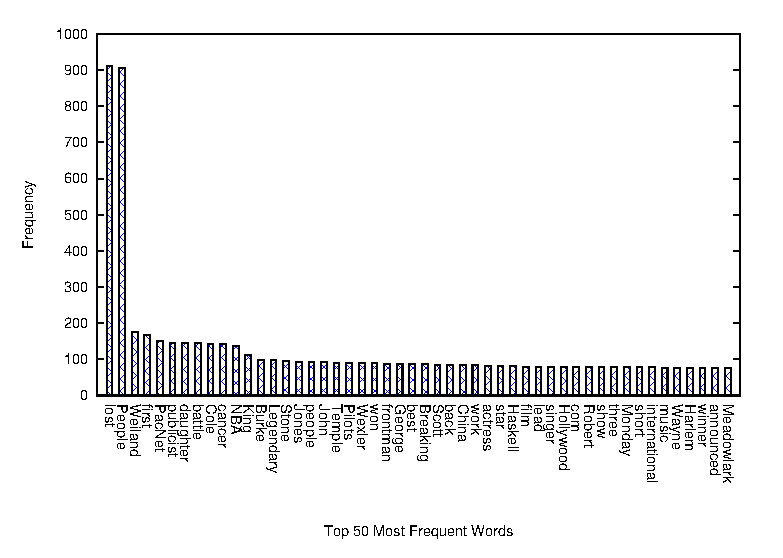
\includegraphics[scale=1.1] {Plots/wordFreq_allArticles.eps}
 \caption {Words vs Frequency}
 \end{center}
\end{figure}



\section{\textbf{Feature Selection}}
\textit{Q 2. Convert them to data matrix (each row is an article and each column is a unique term).}\\

In this section, I present the details of forming a data matrix where each row is an article and each column is a unique word. Please refer script \textbf{cnnProject1/dataMatrix.py} for the implementation details.

\begin{itemize}[label={}]

\item \textbf{Step 1: }  I filtered out following words from the data retrieved from each article

\textit{['many', 'not' ,'into', 'long' , 'Sunday' , 'Thursday' ,'Thu', 'Then' , 'Saturday' , 'then', 'They' , 'both' , 'whose' ,'New' , 'played'  ,'January' , 'February', 'March', 'April', 'May', 'June', 'July' , 'August', 'September' , 'October' , 'November' , 'December','Photos' ,'Whose' , 'had' ,'according','Dow', 'She', 'after' ,'known', 'age' , 'its' , 'have' , 'can' , 'were' ,'are' , 'all' , 'Sat' , 'just' , 'like' , 'he' , 'her' , 'him' , 'from' , 'from' ,'one' , 'will' ,'his' , 'Sans' , 'said' , 'that' , 'who' , 'contributed' ,'cnn', 'cable' , 'Network' , 'Reserved' , 'CNN' ,'Updated' , 'unfold' , 'preference' , 'Set' , 'unfolds' , 'network' , 'News', 'Cable' , 'unfolds.', 'preference:' ,'is' ,'as' ,'with' , 'Find', 'out', 'happening', 'world', 'world', 'ET,', 'Chat', 'Facebook', 'Messenger' , 'Messenger.' , 'world', '2015','unfolds.', 'Rights', 'Reserved.' ,'edition', 'preference:' , 'edition', 'it' , 'a' , 'are', 'an' , 'The' , 'has' , 'the' ,  'on' , 'A' , 'which' , 'under' , 'to' , 'you', 'provided', 'All' , 'this' , 'u' , 'us' , 'of' , 'was' , 'Mr.' , 'y' , 'Find', 'out', 'what', 'happening', 'world', 'world', 'ET,', 'Chat', 'Facebook', 'Messenger' , 'Messenger.' , 'world', '2015','unfolds.' , 'Rights', 'Reserved.' ,'edition', 'preference:' , 'edition', 'it' , 'a' , 'are', 'an' , 'The' , 'has' , 'for' , 'in' , 'the' , 'is' , 'on' , 'A' , 'which' , 'under' , 'to' , 'you', 'provided', 'All' , 'this' , 'u' , 'us' , 'of' , 'and' , 'was' , 'or' , 'y']}

\item \textbf{Step 2:} I sorted the list of words in decreasing order of its frequency. (only until I get first  top K frequent unique words).

\item \textbf{Step 3:} I created a data matrix of size (Number of Articles) X (Top K Most Frequent Words). Each cell contains the frequency of each unique word (Column) for following article (Row).

\end{itemize}

\section{\textbf{Similarity Metrics}}
\textit{Q 3. Compute the similarity between each pair of articles with Euclidean distance (you need to
convert the Euclidean distance to similarity), Cosine and Jaccard.}\\

In this section, I describe how I computed the similarity between each pair of articles with Euclidean distance, Cosine and Jaccard.

\subsection{Euclidean Similarity:}

For a pair of articles say, Article(i) = $\{w_{i0}, w_{i1}, \dots w_{i(K-1)} \}$ and Article(j) = $\{w_{j0}, w_{j1}, \dots w_{j(K-1)} \}$, the euclidean similarity $E(ij)$ is given by

\begin{equation} 
E(ij) = \frac{1}{1 + \sqrt{(Article(i) - Article(j))^2}}
\end{equation}

\begin{equation}\label{euclid}
E(ij) = \frac{1}{1 + \sqrt{(w_{j0} - w_{i0})^2 + \dots + (w_{j(K-1)} - w_{i(K-1)})^2  }}
\end{equation}

\textbf{Example }Consider Article(1) = $\{0, 2, 1\}$ and Article(2) = $\{2, 1, 0\}$, then
\begin{itemize}[label={}]
\item $( Article(1) - Article(2))^2$ = $ (0 -2) ^2 + (2 - 1)^2 + (1 - 0)^2 = 6$

\end{itemize}

$$ E(12) = \frac{1}{1 + \sqrt{6}} = 0.14$$

\subsection{Cosine Similarity:}

For a pair of articles say, Article(i) = $\{w_{i0}, w_{i1}, \dots w_{i(K-1)} \}$ and Article(j) = $\{w_{j0}, w_{j1}, \dots w_{j(K-1)} \}$, the cosine similarity $C(ij)$ is given by

\begin{equation}
E(ij) = \frac{Article(i) Article(j)}{||Article(i)|| . ||Article(j)||}
\end{equation}

\begin{equation}\label{cosine}
E(ij) = \frac{(w_{j0} - w_{i0}) + \dots + (w_{j(K-1)} - w_{i(K-1)}) }{\sqrt{(w_{i0}w_{i0} + \dots + w_{i(K-1)}w_{i(K-1)})} \sqrt{(w_{j0}w_{j0} + \dots + w_{j(K-1)}w_{j(K-1)})}}
\end{equation}

\textbf{Example}  Consider Article(1) = $\{0, 2, 1\}$ and Article(2) = $\{2, 1, 0\}$, then
\begin{itemize}[label={}]

\item Article(1).Article(2) = $ 0.2 + 2.1 + 1.0$ = $2$
\item $||$Article(1)$||$ = $\sqrt{0.0 + 2.2 + 1.1}$ = $\sqrt{5}$
\item $||$Article(2)$||$ = $\sqrt{2.2 + 1.1 + 0.0}$ = $\sqrt{5}$

\end{itemize}

$$C(12) = \frac{2}{\sqrt{5}.\sqrt{5}} = \frac{2}{5} = 0.4$$
\subsection{Jaccard Similarity:}
For a pair of articles say, Article(i) = $\{w_{i0}, w_{i1}, \dots w_{i(K-1)} \}$ and Article(j) = $\{w_{j0}, w_{j1}, \dots w_{j(K-1)} \}$, the jaccard similarity $J(ij)$ is given by

\begin{equation}\label{jaccard}
J(ij) = \frac{Article(i) \cap Article(j)}{Article(i) \cup Article(j)}
\end{equation}


\textbf{Example: } Consider Article(1) = $\{0, 2, 1\}$ and Article(2) = $\{2, 1, 0\}$, then

\begin{itemize}[label={}]
\item $w_{11} \cap w_{21} = 0$  and $w_{11} \cup w_{21} = 2$ 
\item $w_{12} \cap w_{22} = 1$ and $w_{12} \cup w_{22} = 2$ 
\item $w_{13} \cap w_{23} = 0$ and $w_{13} \cup w_{23} = 1$ 
\end{itemize}

$$ J(12) = \frac{0 + 1 + 0}{2 + 2 + 1} = \frac{1}{5} = 0.2$$




\section{\textbf{ Analysis}}

\textit{Q 4.  Sort all pairs from most similar to least similar based on each of the three types of similarity
measurements } \textit{Q 5. Compare the sorted pairs and discuss which one is more accurate (i.e., close to your own judgment)}

In this section, we first present the correlation between different similarity metrics followed by experimental analysis for pairwise articles similarity measurements based on each of aforestated three similarity metrics.

\subsection{Correlation between different metrics}

\begin{figure}[hb]
\begin{center}
 \subfigure[\label{euclid_jaccard}]{
 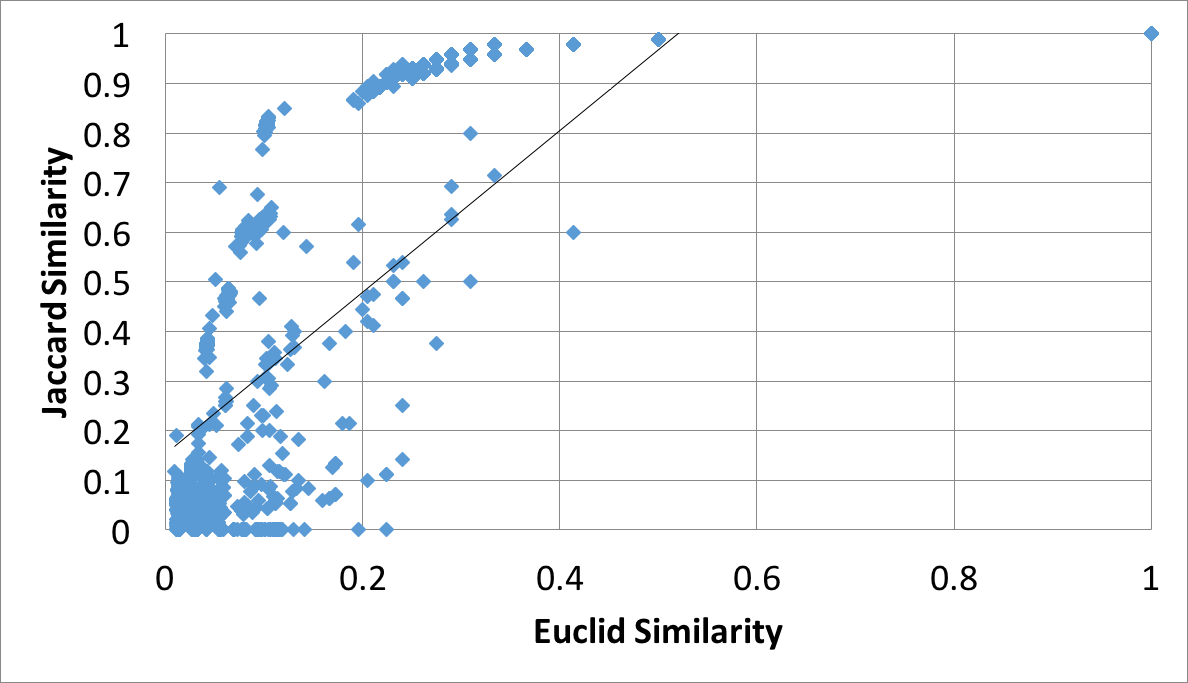
\includegraphics[width = 8cm, height = 4.5cm] {Plots/euclidVsJaccard.png}}
  \subfigure[\label{cosine_jaccard}]{
 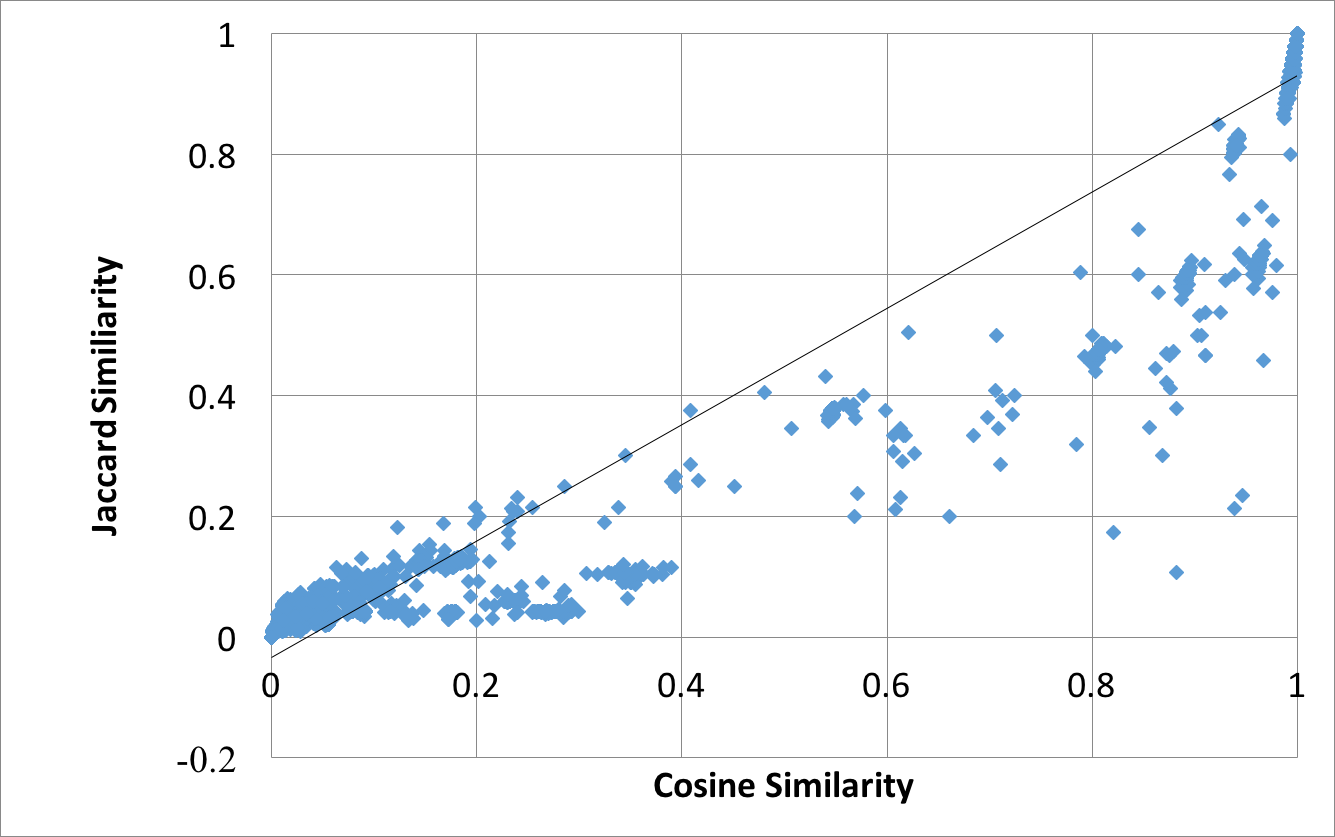
\includegraphics[width =8cm, height = 4.5cm] {Plots/cosineVsJaccard.png}}
 \subfigure[\label{euclid_cosine}]{
 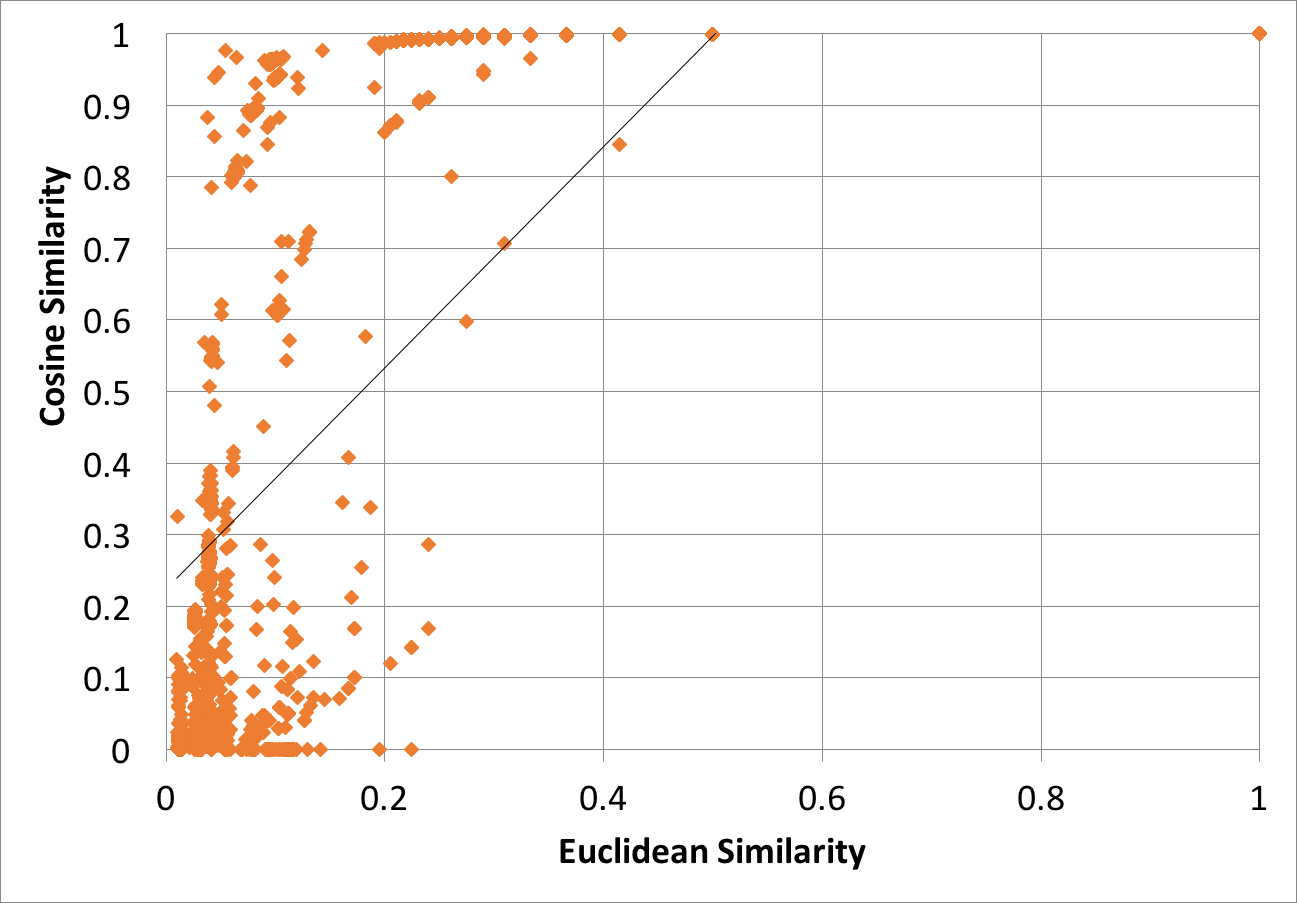
\includegraphics[width = 8cm, height = 4.5cm] {Plots/euclidVsCosine.png}}
\caption{  a. Euclid vs Jaccard b. Cosine vs Jaccard c. Euclid vs Cosine}
\end{center}
\end{figure}

As shown in Fig. \ref{euclid_jaccard}, \ref{cosine_jaccard} and \ref{euclid_cosine}, it is evident that for the given dataset, the cosine and jaccard have high correlation and compute similar  similarity values for most of the article pairs. Whereas, the euclidean similarity computes different similarity value for each article pair than compared to its counterparts.
 

 Fig. \ref{usecase1} shows the non-increasing order of similarity score achieved based on all three Euclidean, Cosine and Jaccard metrics. From here also, it is evident that cosine and jaccard metrics are highly correlated. Whereas, euclidean one is not. Also, the highest score achieved in cosine and jaccard is 1 whereas in case of euclidean, it is almost $0.5$. Also, it is not  very sensitive to the variation of similarity scores for different article pairs. This also suggests that the euclidean is not a good metric for similarity measurement for aforementioned data set.
 
  
\begin{figure}[h]
\begin{center}
 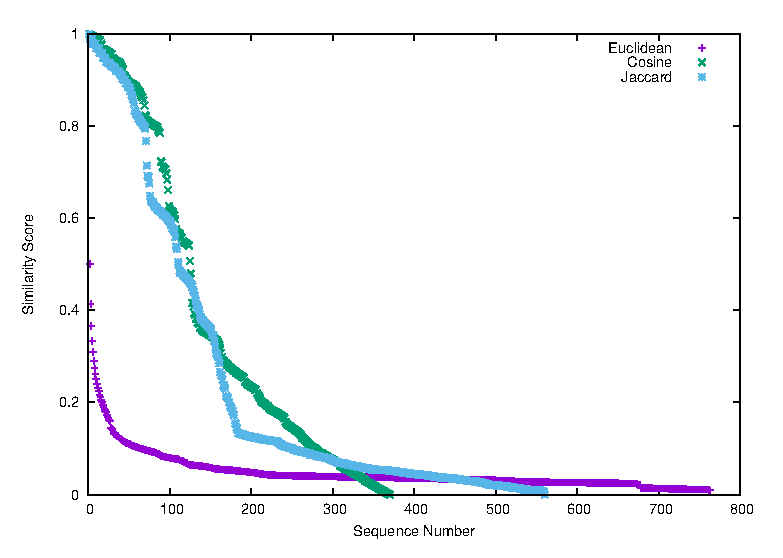
\includegraphics[scale=.90] {Plots/similarityUsecase.eps}
 \caption {Similarity Metrics: Maximum to Minimum Score }\label{usecase1}
 \end{center} 
\end{figure}


\subsection{Article pair similarity analysis}


\subsubsection{\textbf{Analysis of Euclidean Metric}}

As shown in Fig. \ref{euclidean_1} and \ref{euclidean_2}, the euclidean similarity score for most of the article pairs range from $0$ to $0.5$ which is also evident from Fig. \ref{euclidean_3}. This is because for any considered article pair, the frequency of unique words are usually very high (belonging to its respective article), hence the euclidean distance for an article pair is usually high (thus, the euclidean similarity score is low.)


\begin{figure*}[h]
\begin{center}
\label{thr}
\subfigure[\label{euclidean_1}]{
\epsfig{figure=Plots/unsortedEuclideanSimilarity.eps,width=3.40in,keepaspectratio}}
\subfigure[\label{euclidean_2}]{
\epsfig{figure=Plots/unsortedEuclideanSimilarity2D.eps,width=3.40in,keepaspectratio}}
\subfigure[\label{euclidean_3}]{
\epsfig{figure=Plots/sortedEuclideanSimilarity.eps,width=4.00in,keepaspectratio}}
\caption{  Euclidean Similarity: a. 3D View  b. Surface (Map) View  c. Unique Euclidean Similarity Score (Sorted)}
\end{center}
\end{figure*}

\iffalse
\begin{figure}[h] \label{euclidean_3}
\begin{center}
 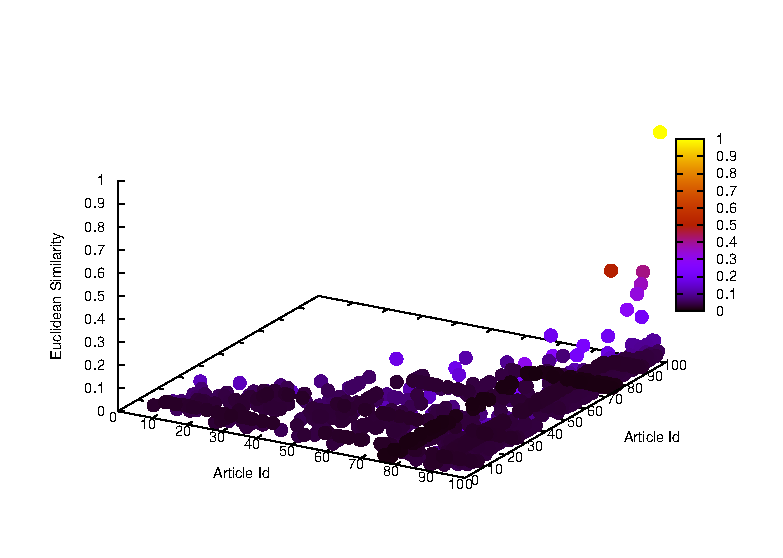
\includegraphics[scale=.90] {Plots/sortedEuclideanSimilarity.eps}
 \caption {Unique Euclidean Similarity Score (Sorted)}
 \end{center}
\end{figure}

\fi

\subsubsection{\textbf{Analysis of Cosine Metric}}
As shown in Fig. \ref{cosine_1} and \ref{cosine_2}, the cosine similarity score varies from $0$ to $1$. Here, it is important to observe that the there are comparatively very high number of article pairs which have high similarity score  (close to $1$). This similarity is capable of finding better similarity scores between any given article pair because it takes both the existence of unique words (direction) and frequency of words (magnitude) into consideration. Hence, this one seems to work best.

Fig. \ref{cosine_3} shows the distribution of unique similarity score for all article pairs based on cosine metric. It also verifies that cosine metric is able to better determine the similarity scores for any article pair.

\begin{figure}[h]
\begin{center}
\label{thr}
\subfigure[\label{cosine_1}]{
\epsfig{figure=Plots/unsortedCosineSimilarity.eps,width=3.40in,keepaspectratio}}
\subfigure[\label{cosine_2}]{
\epsfig{figure=Plots/unsortedCosineSimilarity2D.eps,width=3.40in,keepaspectratio}}
\subfigure[\label{cosine_3}]{
\epsfig{figure=Plots/sortedCosineSimilarity.eps,width=3.40in,keepaspectratio}}
\caption{  Cosine Similarity: a. 3D View  b. Surface (Map) View c. Unique Cosine Similarity Score (Sorted)}
\end{center}
\end{figure}

\iffalse
\begin{figure}[h] \label{cosine_3}
\begin{center}
 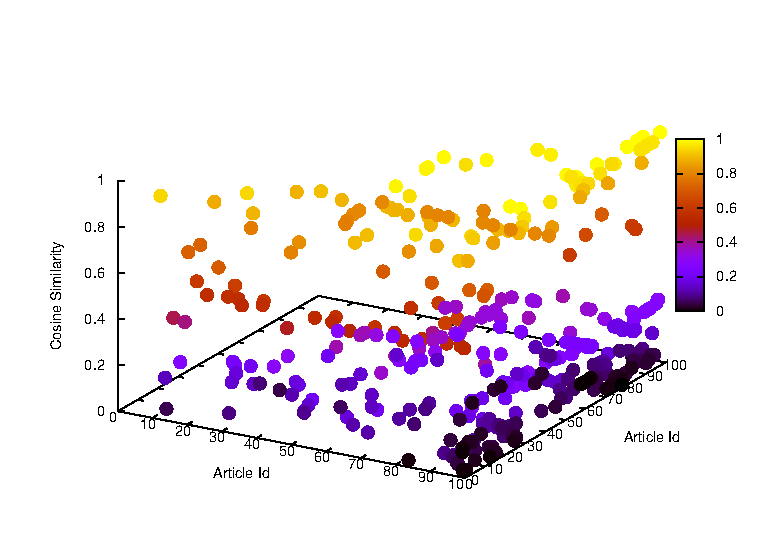
\includegraphics[scale=.90] {Plots/sortedCosineSimilarity.eps}
 \caption {Unique Cosine Similarity (Sorted)}
 \end{center}
\end{figure}
\fi



\begin{figure}[h]
\begin{center}
\label{thr}
\subfigure[\label{jaccard_1}]{
\epsfig{figure=Plots/unsortedJaccardSimilarity.eps,width=3.40in,keepaspectratio}}
\subfigure[\label{jaccard_2}]{
\epsfig{figure=Plots/unsortedJaccardSimilarity2D.eps,width=3.40in,keepaspectratio}}
\subfigure[\label{jaccard_3}]{
\epsfig{figure=Plots/sortedJaccardSimilarity.eps,width=3.40in,keepaspectratio}}
\caption{ Jaccard Similarity: a. 3D View b. Surface (Map) View c. Unique Jaccard Similarity Scores (Sorted)}
\end{center}
\end{figure}

\iffalse
\begin{figure}[h] \label{jaccard_3}
\begin{center}
 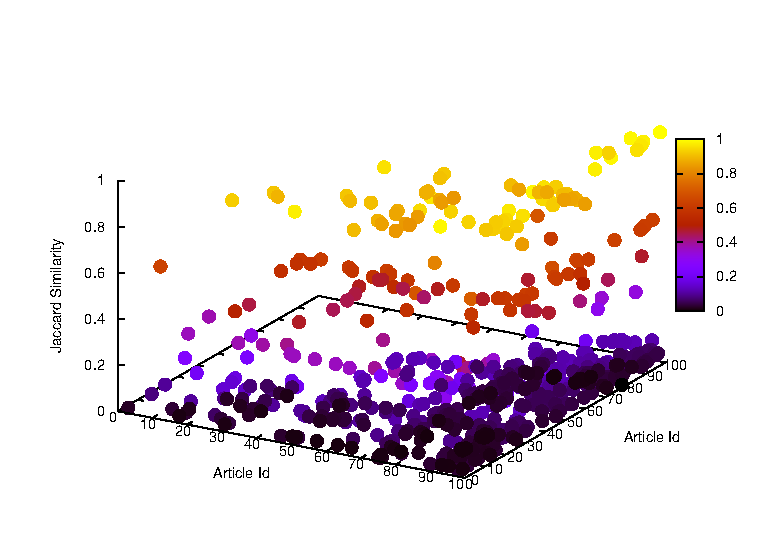
\includegraphics[scale=.90] {Plots/sortedJaccardSimilarity.eps}
 \caption {Unique Jaccard Similarity Scores (Sorted)}
 \end{center}
\end{figure}
\fi

\subsubsection{ \textbf{Analysis of Jaccard Metric}}
Fig \ref{jaccard_1} and \ref{cosine_2} show that similarity scores based on jaccard metric also work as better as that of cosine metric. It is also evident from aforementioned correlation between cosine and jaccard metrics (refer Fig. \ref{cosine_jaccard}).

Fig. \ref{cosine_3} shows the distribution of unique similarity values calculated based on Jaccard metric for all article pairs. It also shows that Jaccard works very well for computing similarity values between each article pair.


\subsubsection{\textbf{Comments}} From the above experimental analysis, it is clear that cosine and Jaccard metrics are suitable metrics for the determination of similarity values for any given pair of articles in the considered data set. Both are sensitive to the variation in similarity score for a varying set of article pairs since the value ranges from 0 to 1. Whereas, the euclidean similarity does not perform very well in both instances. It is also intuitive as cosine metric considers both direction and magnitude for the computation of similarity score for a given article pair. Similarly, Jaccard metric considers both the number of common unique words as well as the frequency of each common unique word.  In contrast, the euclidean metric only considers the distance between the pair of articles. 

\end{document}